\newcommand{\DoNotLoadEpstopdf}{}
\documentclass[11pt,letterpaper]{article}
\usepackage[T1]{fontenc}
\usepackage[utf8]{inputenc}
\usepackage[margin=.86in,top=.82in,bottom=.84in,headheight=24pt,headsep=.21in]{geometry}
\usepackage{amsmath,amssymb,amsthm,mathtools}
\usepackage{mathpazo,helvet,microtype}
\usepackage{booktabs,tabularx,array,longtable,multirow}
\usepackage{graphicx,xcolor,tikz,pgfplots}
\usetikzlibrary{arrows.meta,positioning,calc,fit,backgrounds,decorations.pathmorphing}
\pgfplotsset{compat=1.18}
\usepackage[most]{tcolorbox}
\usepackage{enumitem,needspace,fancyhdr,titlesec,caption,float,placeins}
\usepackage{listings,xurl,upquote}
\usepackage[numbers,sort&compress]{natbib}
\usepackage[unicode,bookmarksnumbered]{hyperref}
\usepackage{bookmark}
\definecolor{Ink}{HTML}{231629}
\definecolor{Plum}{HTML}{482847}
\definecolor{Wine}{HTML}{742E50}
\definecolor{Gold}{HTML}{A7792E}
\definecolor{LightGold}{HTML}{E9C882}
\definecolor{Ivory}{HTML}{FCF9F2}
\definecolor{Sea}{HTML}{1D786F}
\definecolor{SeaLight}{HTML}{A0E1CE}
\definecolor{Muted}{HTML}{655E6A}
\definecolor{Rule}{HTML}{DACFBD}
\definecolor{Pale}{HTML}{F3EEF5}
\hypersetup{pdftitle={SURF THE EXPONENTIAL: The Missing Move},pdfauthor={Vincent Boucher},pdfsubject={From verified criticism to new capabilities, viable markets, and better inventors},pdfkeywords={Transformational Intelligence, Alpha Genesis Flywheel Omega, frontier replay, counterexamples, invention, evidence, market construction},colorlinks=true,linkcolor=Plum,citecolor=Plum,urlcolor=Sea}
\ifdefined\pdfinfoomitdate\pdfinfoomitdate=1\fi
\ifdefined\pdftrailerid\pdftrailerid{}\fi
\ifdefined\pdfsuppressptexinfo\pdfsuppressptexinfo=15\fi
\pagestyle{fancy}\fancyhf{}
\fancyhead[L]{\footnotesize\sffamily\color{Muted}SURF THE EXPONENTIAL}
\fancyhead[R]{\footnotesize\sffamily\color{Muted}The Missing Move \;|\; Boucher}
\fancyfoot[L]{\scriptsize\sffamily\color{Muted}ALPHA GENESIS FLYWHEEL $\Omega$}
\fancyfoot[R]{\small\color{Gold}\thepage}
\renewcommand{\headrulewidth}{.35pt}
\renewcommand{\headrule}{\hbox to\headwidth{\color{Rule}\leaders\hrule height \headrulewidth\hfill}}
\setlength{\parindent}{0pt}\setlength{\parskip}{.47em plus .06em minus .04em}
\setlength{\emergencystretch}{2.6em}\linespread{1.035}\raggedbottom
\widowpenalty=10000\clubpenalty=10000
\titleformat{\section}{\Large\bfseries\color{Plum}}{\color{Gold}\thesection}{.7em}{}
\titleformat{\subsection}{\large\bfseries\color{Ink}}{\thesubsection}{.7em}{}
\titleformat{\subsubsection}{\normalsize\bfseries\color{Ink}}{\thesubsubsection}{.7em}{}
\titlespacing*{\section}{0pt}{2.2ex plus .5ex minus .2ex}{.8ex}
\titlespacing*{\subsection}{0pt}{1.6ex plus .4ex minus .2ex}{.5ex}
\captionsetup{font=small,labelfont={bf,color=Plum},textfont={color=Muted},skip=7pt}
\setlist{leftmargin=1.45em,itemsep=.14em,topsep=.2em,parsep=0pt}
\renewcommand{\arraystretch}{1.16}
\newcolumntype{Y}{>{\raggedright\arraybackslash}X}
\newcolumntype{P}[1]{>{\raggedright\arraybackslash}p{#1}}
\newcommand{\E}{\mathbb{E}}\newcommand{\Prob}{\mathbb{P}}\newcommand{\I}{\mathcal{I}}
\newcommand{\F}{\mathcal{F}}\newcommand{\B}{\mathcal{B}}\newcommand{\D}{\mathcal{D}}
\DeclareMathOperator*{\argmax}{arg\,max}
\newtheorem{definition}{Definition}[section]
\newtheorem{proposition}{Proposition}[section]
\newtheorem{corollary}{Corollary}[section]
\theoremstyle{remark}\newtheorem{remark}{Remark}[section]
\newtcolorbox{thesisbox}{enhanced,breakable,colback=Ivory,colframe=Gold,boxrule=.5pt,arc=1.4mm,left=12pt,right=12pt,top=9pt,bottom=9pt,before skip=10pt,after skip=10pt}
\newtcolorbox{statusbox}{enhanced,breakable,colback=Pale,colframe=Plum,boxrule=0pt,borderline west={2.5pt}{0pt}{Plum},arc=0mm,left=11pt,right=11pt,top=8pt,bottom=8pt,before skip=9pt,after skip=9pt}
\newtcolorbox{seabox}{enhanced,breakable,colback=Sea!5,colframe=Sea,boxrule=0pt,borderline west={2.5pt}{0pt}{Sea},arc=0mm,left=11pt,right=11pt,top=8pt,bottom=8pt,before skip=9pt,after skip=9pt}
\newcommand{\smallhead}[1]{\par\smallskip{\sffamily\bfseries\color{Gold}#1}\par\smallskip}
\lstset{upquote=true,basicstyle=\small\ttfamily,breaklines=true,columns=fullflexible,keepspaces=true,showstringspaces=false,frame=single,rulecolor=\color{Rule},backgroundcolor=\color{Ivory},framesep=7pt}
\setcounter{tocdepth}{1}
\begin{document}
\begin{titlepage}
\thispagestyle{empty}

\begin{tikzpicture}[remember picture,overlay]
\fill[Ink] (current page.south west) rectangle (current page.north east);
\fill[Plum] ([yshift=2.2in]current page.south west) rectangle ([yshift=-4.0in]current page.north east);
\draw[LightGold,opacity=.75,line width=.6pt] ([xshift=.36in,yshift=.36in]current page.south west) rectangle ([xshift=-.36in,yshift=-.36in]current page.north east);
\node[anchor=north west,text=LightGold,font=\sffamily\small] at ([xshift=.73in,yshift=-.65in]current page.north west) {MONTREAL.AI\quad /\quad QUEBEC.AI};
\node[anchor=north east,text=LightGold,font=\sffamily\small] at ([xshift=-.73in,yshift=-.65in]current page.north east) {RESEARCH 1.0.0};
\node[anchor=north,text=Ivory,font=\sffamily\fontsize{19}{23}\selectfont] at ([yshift=-1.28in]current page.north) {SURF THE};
\node[anchor=north,text=LightGold,font=\fontsize{43}{48}\selectfont\bfseries] at ([yshift=-1.78in]current page.north) {EXPONENTIAL};
\node[anchor=north,text=Ivory,font=\fontsize{28}{34}\selectfont] at ([yshift=-2.65in]current page.north) {The Missing Move};
\node[anchor=north,align=center,text=Ivory,text width=6.7in,font=\fontsize{14}{19}\selectfont] at ([yshift=-3.36in]current page.north) {From Verified Criticism to New Capabilities,\\Viable Markets, and Better Inventors};
\begin{scope}[shift={([xshift=.72in,yshift=3.12in]current page.south west)},x=1in,y=1in]
\foreach \i in {0,...,14}{
  \pgfmathsetmacro{\off}{\i*.057}
  \draw[SeaLight,opacity=.16,line width=.45pt] (0,\off) .. controls (1.3,.05+\off) and (1.9,.18+\off) .. (2.7,.55+\off) .. controls (3.4,.90+\off) and (4.4,1.93+\off) .. (5.08,1.74+\off) .. controls (5.5,1.62+\off) and (5.72,.92+\off) .. (6.93,1.09+\off);
}
\draw[LightGold,line width=1.5pt] (0,.4) .. controls (1.3,.4) and (1.9,.58) .. (2.7,.95) .. controls (3.35,1.28) and (3.83,1.77) .. (4.15,1.98);
\draw[LightGold,densely dashed,line width=1pt] (4.15,1.98) .. controls (4.6,2.25) and (4.92,2.17) .. (5.22,1.94);
\draw[LightGold,line width=1.5pt] (5.22,1.94) .. controls (5.65,1.58) and (5.7,1.2) .. (6.93,1.49);
\fill[LightGold] (4.15,1.98) circle (2.5pt);\fill[SeaLight] (5.22,1.94) circle (2.5pt);
\node[text=LightGold,font=\sffamily\scriptsize,align=center] at (4.65,2.66) {THE MISSING MOVE};
\draw[LightGold,opacity=.55] (4.65,2.49)--(4.65,2.23);
\node[text=Ivory,font=\fontsize{56}{60}\selectfont] at (1.05,1.76) {$\infty$};
\end{scope}
\node[anchor=north,align=center,text=Ivory,text width=6.6in,font=\fontsize{18}{23}\selectfont] at ([yshift=-8.12in]current page.north) {Find what the answer missed.\\\textcolor{LightGold}{Build what the world is missing.}};
\node[anchor=south west,text=Ivory,align=left,font=\normalsize] at ([xshift=.73in,yshift=.78in]current page.south west) {\textbf{Vincent Boucher}\\Montr\'{e}al, Qu\'{e}bec, Canada};
\node[anchor=south east,text=LightGold,align=right,font=\small] at ([xshift=-.73in,yshift=.78in]current page.south east) {TRANSFORMATIONAL INTELLIGENCE $\infty$\\5 November 2026};
\end{tikzpicture}
\null
\end{titlepage}
\setcounter{page}{1}
\begin{center}
{\small\sffamily\bfseries\color{Gold}ALPHA GENESIS FLYWHEEL $\Omega$}\par\vspace{.12in}
{\LARGE\bfseries\color{Plum}SURF THE EXPONENTIAL}\par\vspace{.07in}
{\Large The Missing Move}\par\vspace{.1in}
{\large From Verified Criticism to New Capabilities,\\Viable Markets, and Better Inventors}\par\vspace{.16in}
\textbf{Vincent Boucher}\quad$\cdot$\quad MONTREAL.AI / QUEBEC.AI\\
{\small Montr\'{e}al, Qu\'{e}bec, Canada\quad$\cdot$\quad 5 November 2026}
\end{center}
\smallhead{ABSTRACT}
A fluent answer can conceal a consequential omission. Asking another model to locate a specific, source-grounded failure can make that omission easier to inspect, but neither disagreement nor agreement establishes truth. We develop this observation into a research architecture for \emph{constructive challenge}: use independently adjudicated criticisms to discover what must be learned, built, coordinated, or changed for a valuable outcome to become attainable. Building on \emph{Transformational Intelligence}, \emph{ALPHA GENESIS FLYWHEEL $\Omega$}, and \emph{Invent the Economy}, the object of challenge expands from a candidate answer to its opportunity set and its means of obtaining evidence. A challenge carries a scoped witness; a proposed response carries a construction and a discriminating test; an economic claim additionally requires voluntary participation, complete costs, and a feasible cash path. We distinguish correction from capability construction, capability construction from market realization, and inherited capability from improved discovery. Conditional analysis shows how false criticism, shared blind spots, adjudication quality, and verification costs determine whether an additional critic is useful. A compact executable reference study checks these relationships and preserves cases in which a stipulated conventional-review comparator ties or wins and retaining the incumbent has greater modeled value. These are authored finite-model results, not measurements of frontier-model discovery or real commercial performance. The empirical programme compares direct execution, self-review, independent challenge, evidence-preserving production, and competent conventional construction on fresh complete campaigns. The ambition is an enterprise that turns the accelerating frontier into newly verified productive possibilities, while making every claimed step of that transformation independently testable.
\begin{statusbox}
\textbf{Research status.} An original synthesis, conditional propositions, executable authored reference models, and a prospective evaluation protocol. Model rates, utilities, prices and costs in the reference study are stipulated inputs. Assisted adversarial review of this manuscript is editorial quality control, not an independent scientific experiment. Exponential enterprise growth, autonomous market invention, actual revenue and improved discovery remain hypotheses requiring their own evidence.
\end{statusbox}
{\small\textbf{Keywords:} transformational intelligence; consequential omissions; counterexamples; constructive challenge; frontier replay; market formation; discovery methods.}
\clearpage
\smallhead{THE PAPER AT A GLANCE}
\begin{thesisbox}
\Large\bfseries\raggedright A verified criticism can expose\\the missing means of a valuable possibility.
\end{thesisbox}
Imagine that an AI summarizes a book beautifully. Another AI finds a passage that changes the meaning of its conclusion. You now have something concrete to inspect. The useful object is the \emph{evidence-backed discrepancy}, not the fact that two systems disagree.

Now apply the same question to an invention or an enterprise. What important condition has the proposal missed? Which useful route did it never consider? What new instrument would let us find out? An answer can be correct within its assumptions while those assumptions exclude the most valuable possibility.
\begin{seabox}
\textbf{The missing move may be a fact to recover, an experiment to run, a capability to construct, or an arrangement that makes voluntary cooperation worthwhile.}\par
The central job is to establish which one it is, build the appropriate response, and test the complete consequence.
\end{seabox}
\begin{center}
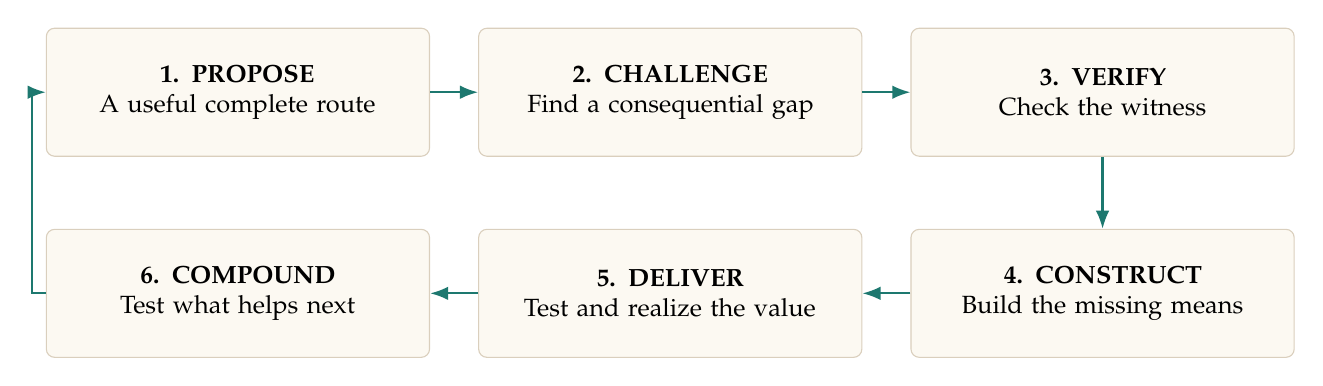
\begin{tikzpicture}[node distance=.36in and .24in, every node/.style={font=\small,align=center},box/.style={draw=Rule,fill=Ivory,rounded corners=3pt,text width=1.75in,minimum height=.64in,inner sep=6pt},arr/.style={-{Latex[length=2.3mm]},line width=.8pt,color=Sea}]
\node[box] (a) {\textbf{1. PROPOSE}\\A useful complete route};
\node[box,right=of a] (b) {\textbf{2. CHALLENGE}\\Find a consequential gap};
\node[box,right=of b] (c) {\textbf{3. VERIFY}\\Check the witness};
\node[box,below=of c] (d) {\textbf{4. CONSTRUCT}\\Build the missing means};
\node[box,left=of d] (e) {\textbf{5. DELIVER}\\Test and realize the value};
\node[box,left=of e] (f) {\textbf{6. COMPOUND}\\Test what helps next};
\draw[arr] (a)--(b);\draw[arr] (b)--(c);\draw[arr] (c)--(d);\draw[arr] (d)--(e);\draw[arr] (e)--(f);\draw[arr] (f.west)--++(-.18,0)|-(a.west);
\end{tikzpicture}
\end{center}
{\small\color{Muted}A useful organizing loop, not a mandatory ceremony. At any stage the best response may be an existing solution, a cheaper test, a simpler formulation, a deferred decision, or stopping.}

\smallhead{THREE QUESTIONS THAT REACH BEYOND DEBATE}
\textbf{Challenge the answer.} What would make this claim wrong or incomplete in a way that matters?\par
\textbf{Challenge the possibilities.} What valuable route is absent from the choices we are comparing?\par
\textbf{Challenge the instrument.} What prevents us from finding out, and can we construct better evidence?

\textbf{What would count as progress?} More accepted value after complete costs; fewer consequential missed opportunities and invalid promotions; a specific successor helped by what was retained; and, separately, better discovery on fresh work under matched resources.

\textbf{Read by purpose.} Sections 1--2 give the intuition and construction protocol. Sections 3--4 explain when criticism helps and how evidence can fail. Sections 5--6 connect frontier change to viable productive arrangements. Sections 7--9 supply the exact study, empirical programme and compounding contract. The appendices provide practical templates, proofs and claim boundaries.
\clearpage
\tableofcontents
\clearpage
\section{From a missing chapter to a missing possibility}
\label{sec:opening}
A reader asks a frontier language model to summarize a book. The summary is fluent, balanced in tone, and apparently complete. The reader has not read the book, so the very quality that makes the summary convenient also makes it difficult to verify. A second model receives the book and the summary and is asked to identify a consequential omission. It points to a particular passage, explains why that passage changes the conclusion, and provides enough context for an independent check.

The assessment problem has changed. The reader can investigate a specific discrepancy instead of trying to certify the entire compression from its style. This asymmetry is useful: one decisive example can refute a particular claim even when constructing or evaluating the whole artifact is difficult. The second model can nevertheless be wrong. It may invent a passage, misread a qualification, or complain that a short summary does not contain everything. The task should therefore ask for the strongest \emph{supported} criticism and allow the answer that no consequential defect was established.

This observation has direct precedents. Model-written critiques helped human evaluators find flaws in topic-based summaries in the experiments of Saunders et al.\ \citep{saunders}. Later work on code critics found both useful bug detection and hallucinated criticisms \citep{critic}. The opening of \emph{Transformational Intelligence} already develops the book example, adds independent adjudication, and considers producing a source-grounded structure before compression \citep[\S1 and Appendix C]{boucher_ti}. We build on that foundation rather than claim the second critic as a new invention.

\subsection{The larger omission}
An enterprise faces a related problem with a crucial difference. A book has a finite source. The world does not supply a complete volume containing every possible invention, production process, or voluntary arrangement. A proposal can accurately describe its candidate and still fail to consider a much better route. A scientific investigation can compare its hypotheses carefully while missing an instrument that would change which questions are answerable. An economically sensible rejection can omit a complementary construction that would make the activity viable.

The central research question is therefore:
\begin{thesisbox}
\textbf{Can intelligence turn a consequential, verified gap in what we know or consider into the means of doing something valuable that the current arrangement cannot deliver?}
\end{thesisbox}
The answer requires more than another round of disagreement. A valid objection has to connect to a diagnosis, a response, an executable construction, and a complete comparison. Some objections call for correction. Others call for new evidence. A third class reveals a removable dependency: the current method requires something expensive or unavailable, but an alternative may achieve the same authorized outcome without it. The best response can also be procurement, an established method, or no further action.

Consider a hypothetical small manufacturer that rejects a new product because qualifying each short production run appears too expensive. A failure challenger asks whether its proposed shortcut really establishes the required quality. A possibility challenger asks whether several runs share a testable structure that would make a common qualification instrument worthwhile. An instrument challenger asks whether the existing measurements can distinguish acceptable from unacceptable behavior. These are different questions. Their answers might support a shared test capability, a different production method, or the original rejection. The useful advance is whatever survives construction and evidence.

\subsection{How the three papers fit together}
\begin{table}[htbp]
\small
\begin{tabularx}{\textwidth}{P{1.48in}YY}
\toprule
\textbf{Foundation} & \textbf{What it makes editable} & \textbf{Its role here}\\
\midrule
Transformational Intelligence & Representations, information, dependencies and intermediate means, with the authorized purpose preserved. & Diagnose whether a criticism exposes an avoidable restriction; construct and test another formulation.\\
Alpha Genesis Flywheel $\Omega$ & The conversion of frontier capability into useful possibilities and better discovery methods. & Replay consequential gaps when a relevant capability changes; distinguish better tools from better invention.\\
Invent the Economy & Productive capability and the arrangement of participants, transfers, risk and timed funding. & Build the complete conditions under which useful work is technically valid and voluntarily worthwhile.\\
\bottomrule
\end{tabularx}
\caption{An explicit synthesis of the supplied manuscripts \citep{boucher_ti,boucher_genesis,boucher_economy}. The organizing transition of this manuscript is the move from an adjudicated challenge to a tested productive response.}
\end{table}

\subsection{Contribution and intellectual position}
The paper contributes an operational \emph{Missing Move contract}; a distinction among challenges to an answer, its opportunity set, and its evidence instrument; conditional accounting for useful and harmful criticism; and a matched evaluation programme connecting constructive challenge to frontier adaptation and economic continuation. An executable finite case carries the central transition through: find a consequential information loss, construct a sufficient representation, verify its minimality, and test a changed successor. A separate cash-path counterexample shows why a profitable successful delivery can still leave a promised refund unfunded. The larger architecture remains a proposal.

Counterexample-guided synthesis provides an established model for generating candidates, finding failures, and using those failures to constrain subsequent construction \citep{cegis}. Debate offers a different route to eliciting useful information for a judge \citep{debate}. Neither formal finite-program guarantees nor idealized debate arguments make open-world invention automatically reliable. A natural-language challenge may lack a sound specification, a complete checker, or even an adequate measurement. We make those missing conditions part of the work.

The ambition is expansive without requiring every component to be novel. An ordinary test, a familiar algorithm, or a conventional contracting arrangement can be the decisive missing move. Scientific novelty, useful construction, commercial success, and improvement of discovery have different evidence requirements. A competent institution pursues the valuable result and states precisely which of those achievements it has established.

\section{The Missing Move contract}
\label{sec:contract}
\subsection{Keep purpose, means and measurement distinct}
Let the purpose contract be
\begin{equation}
\I=(O,H,A,B,T),
\end{equation}
where $O$ denotes the intended outcome, $H$ the hard requirements, $A$ the authority to act, $B$ the available resources, and $T$ the relevant time conditions. A formulation $F$ describes a particular set of representations, information procedures, allowed internal actions and intermediate targets. An evaluation instrument $E$ supplies evidence about whether a realization serves $\I$. This separation follows the foundational manuscript \citep[\S2]{boucher_ti}.

A critic may propose changing $F$ or improving $E$. It cannot silently amend $O$, weaken $H$, expand $A$, or spend imaginary resources. If the required deliverable is a two-page summary, an interactive application does not fulfill the instruction merely because it might be more interesting. If the purpose is to understand an argument before a meeting, the application may be a legitimate alternative. The distinction depends on the actual assignment. A broad discovery charter may authorize proposing new beneficiary outcomes within a stated mission. Once a candidate enters confirmation, freeze its concrete outcome contract; a material change of ends or permissions begins an explicitly amended comparison.

\begin{definition}[Consequential challenge]
Relative to a stated purpose and decision, a consequential challenge is an allegation that a candidate claim, omitted condition, excluded alternative, or inadequate evidence procedure could materially change the required outcome or a justified choice of action. It is a hypothesis until its relevant evidence and materiality are adjudicated.
\end{definition}
An omission is therefore not automatically a defect. A summary must compress; an engineering plan must abstract; a research portfolio must leave possibilities unexplored. Materiality depends on the user's purpose, the decision at stake, and the available budget. Exhaustive commentary can make a useful artifact worse.

\begin{seabox}
\textbf{A missing distinction you can inspect.} A report stores only the mean of two readings and claims it can determine whether every reading is at most 90. The traces $(60,100)$ and $(80,80)$ have the same mean, 80, but opposite acceptance outcomes. That pair is a concrete witness against the claim. Retaining the maximum before compression is an ordinary sufficient response; it does not recover an already discarded maximum. Section~\ref{sec:construction} makes the transition from this witness to a constructed representation and a changed successor executable. The point is visible: a missing distinction becomes a specific construction target.
\end{seabox}

\subsection{Two linked records: the challenge and the construction}
We separate a challenge record $w$ from a response record $r$. This prevents the correctness of a diagnosis from being mistaken for the correctness of its favorite remedy:
\begin{align}
 w &= (c,s,e,m,q),\\
 r &= (\rho,F',k,\tau,v).
\end{align}
Here $c$ identifies the challenged claim or choice; $s$ fixes its scope and source versions; $e$ is inspectable evidence; $m$ states decision materiality; and $q$ gives a falsifying or discriminating check. The response identifies the diagnosed restriction $\rho$, alternative formulation $F'$, executable construction $k$, complete test $\tau$, and validity and invalidation conditions $v$.

For a book, $e$ may be an accurately located passage with enough surrounding context to preserve its meaning. For a program, it can be an executable input and failing output. For a market arrangement, it may be a feasible participant deviation, an omitted liability, or a cash-flow prefix that cannot be funded. For a scientific instrument, the evidence may show that two materially different states are observationally indistinguishable under the proposed measurement procedure. Each domain needs its own semantics of evidence.

\begin{table}[htbp]
\small
\begin{tabularx}{\textwidth}{P{1.25in}YY}
\toprule
\textbf{Question} & \textbf{Minimum useful answer} & \textbf{What it cannot establish alone}\\
\midrule
What is challenged? & An exact assertion, required property or excluded route. & That the complete candidate is bad.\\
Where is the evidence? & Source identity and location, a runnable witness, or a justified measurement. & That the evidence source is infallible.\\
Why does it matter? & A specified effect on purpose, acceptance or decision. & That every omitted detail deserves repair.\\
What kind of obstacle? & A hard constraint to honor, an uncertain premise to resolve, or a restriction of means to change. & Permission to weaken a real requirement.\\
What is the response? & A buildable alternative plus a test against serious rivals. & That a valid criticism makes the repair valid.\\
When does it transfer? & Preconditions, costs, interfaces and invalidation rules. & Current acceptance or authority for a successor.\\
\bottomrule
\end{tabularx}
\caption{A compact contract for constructive challenge. Evidence and construction are linked while remaining separately accountable.}
\end{table}

\subsection{Three directions of challenge}
\textbf{The failure challenger} searches for a supported reason the proposed route would fail: a contradiction, missing exception, unacceptable operating case, uncompensated participant, or unpriced obligation. Its best output is a decisive witness, not a large number of objections.

\textbf{The possibility challenger} constructs a serious alternative the current candidate set excludes. This matters because a selector can choose perfectly among bad proposals. The relevant comparison is between complete routes to the same intended outcome, including an existing solution or doing nothing. A purportedly impossible activity becomes a candidate opportunity only when a concrete response changes the constraint responsible for that judgment.

\textbf{The instrument challenger} examines whether the available evidence can settle the dispute. It may propose a new observation, an independent implementation, a different decomposition, or a validated measure closer to the intended outcome. Its product is a better way to find out. It must itself be tested, with both sides rescored under a common supported instrument when that instrument changes \citep[\S7]{boucher_ti}.

These are functions, not necessarily three agents. One capable system, several systems, a domain expert or conventional software may perform them. Role separation helps organize work; it does not manufacture independent errors or independent evidence.

\subsection{Adjudicate before repair, and compare several responses}
An adjudicator returns one of four useful states: \emph{supported and material}, \emph{supported but immaterial}, \emph{refuted}, or \emph{unresolved}. ``Unresolved'' is not a softer form of acceptance. It identifies an uncertainty that the next decision must either resolve, tolerate explicitly, eliminate through a changed construction, or avoid.

A supported material challenge opens a response set:
\begin{equation}
\mathcal R(w)=\{\text{repair},\ \text{measure},\ \text{construct},\ \text{rearrange},\ \text{adopt},\ \text{defer or stop}\}.
\end{equation}
Assess critics by independently verified material findings and downstream effects, including harmful revisions and wasted effort. Rewarding objection count, rhetorical force or frequency of overturning the producer encourages the wrong behavior. The categories may overlap. A shared instrument and a staged commitment can be jointly useful even when neither alone justifies its cost. A system that immediately repairs the first valid objection can miss a simpler route that removes the disputed dependency altogether. Conversely, adding an elaborate institution to solve a local defect can be worse than a small correction.

\begin{seabox}
\textbf{The constructive question is not only ``What is wrong?''}\par
It is: \textbf{``What would have to become true, available, measurable or mutually worthwhile for the valuable outcome to work---and can we make that happen?''}
\end{seabox}

\subsection{An opportunity witness needs two sides}
A counterexample can demonstrate that a universal assertion is false on a stated case. An opportunity claim needs more. It needs a \emph{positive side}: a complete route that meets the purpose under its stated conditions. It also needs a \emph{comparative side}: why this route matters relative to available alternatives, including a route that reconstructs the supposed missing asset conventionally.

Let $J_\I(x)$ be a declared net-outcome measure for an admissible complete route $x$, and let $\B$ be a disclosed finite, nonempty comparison set. Define
\begin{equation}
\alpha_\I(x;\B)=J_\I(x)-\max_{b\in\B}J_\I(b).
\end{equation}
This is a comparison to $\B$, not a proof about every possible enterprise. If outcomes cannot legitimately be collapsed into one scalar, retain a vector of relevant outcomes and report the actual trade-offs. Hard constraints remain constraints rather than purchasable score penalties.

The strongest formulation-dependent claim adds a justified exclusion: the old setup cannot attain the specified outcome within its defined permissions, information and resources. In real research that exclusion is often unavailable. Then the honest claim is a supported gain over the strongest tested complete alternatives. Neither an unsuccessful search nor a pessimistic first draft proves impossibility.

\section{When is another critic worth its cost?}
\label{sec:value}
\subsection{A conditional accounting identity}
Fix one pre-specified, decision-material defect proposition per episode, relative to a stated purpose and task distribution. Let $F$ denote that this exact proposition is true. Let $D$ denote a criticism alleging this same defect, and let $A_c\subseteq D$ denote acceptance of that allegation followed by its specified response. A flawed candidate can receive a false criticism about a different issue; such mixed-target episodes require a richer event partition and are outside this binary reference model. Define
\begin{align}
\pi&=\Prob(F), & d&=\Prob(D\mid F), & f&=\Prob(D\mid\neg F),\\
 a&=\Prob(A_c\mid D,F), & b&=\Prob(A_c\mid D,\neg F).
\end{align}
The letter $A_c$ here refers to an accepted challenge, not the authority component of $\I$. Let $G=\E[\Delta J\mid F,D,A_c]$ be the expected net utility improvement conditional on accepting a true allegation of this target defect; let $H=-\E[\Delta J\mid\neg F,D,A_c]$ be the expected loss conditional on accepting a false allegation. Both include revision and retesting costs on their respective branches. Let $K$ be the expected incremental cost of criticism and adjudication across all branches, including retrieval, discarded objections, latency and opportunity cost. On a zero-probability conditioning event, use a finite declared kernel value: its weighted contribution is zero, and the distribution does not identify it.

\begin{proposition}[Value of adjudicated challenge]
\label{prop:value}
Suppose branches without an accepted challenge retain incumbent utility before review costs. With the conditional quantities above,
\begin{equation}
\boxed{\Delta U=\pi daG-(1-\pi)fbH-K.}
\label{eq:value}
\end{equation}
For $G>0$ and $H,K\geq0$, the challenge route improves expected utility exactly when
\begin{equation}
\pi daG>(1-\pi)fbH+K.
\label{eq:break}
\end{equation}
\end{proposition}
\begin{proof}
Partition accepted revisions into true and false criticisms. Their probabilities are $\pi da$ and $(1-\pi)fb$ by the chain rule. Multiply by their conditional net effects and subtract the expected review cost. No statistical independence between the producer, critic and adjudicator is required.
\end{proof}

Equation~\eqref{eq:value} is an accounting identity under explicit assumptions. It does not tell us that the inputs are calibrated. Multiplying two models' published marginal benchmark accuracies would not estimate these conditional events. In applications, one must measure the actual joint process on the relevant distribution. A correct diagnosis may lead to a harmful repair, in which case $G$ can be negative and the same accounting identity still applies.

The equation exposes several productive choices. Better source access may improve $d$. A clearer witness may improve adjudication. A smaller repair may reduce harm or cost. A different formulation may reduce the need for recurring criticism. A more expensive critic is justified only when its complete consequences improve the choice. The model therefore supports testing evidence-preserving production and conventional inspection as well as adding models.

\subsection{Confirmation is not coverage}
The probability of a material flaw escaping an \emph{accepted challenge} is
\begin{equation}
\Prob(F\cap\neg A_c)=\pi(1-da).
\label{eq:escape}
\end{equation}
This is not the post-repair defect rate: repairs may fail, and false criticisms may introduce new defects. It isolates a different weakness. Even a perfect adjudicator cannot confirm a flaw that the challenger never proposes. High precision among accepted criticisms can coexist with poor coverage of consequential omissions.

For $m$ critics, detection is $\Prob(\bigcup_{i=1}^{m}D_i\mid F)$. Without a conditional independence assumption, only the basic bounds
\begin{equation}
\max_i\Prob(D_i\mid F)\ \leq\ \Prob\!\left(\bigcup_iD_i\mid F\right)\ \leq\ \min\!\left\{1,\sum_i\Prob(D_i\mid F)\right\}
\end{equation}
hold. Perfectly correlated critics obtain no detection gain by replication. Different model providers may supply useful diversity, but their names do not establish the relevant joint distribution.

An illustrative two-critic calculation makes this concrete. Suppose each critic misses a flaw with probability $m_0$, and the Bernoulli miss indicators have a feasible Bernoulli correlation $\rho$. Then
\begin{equation}
\Prob(\text{both miss})=m_0^2+\rho m_0(1-m_0).
\label{eq:correlation}
\end{equation}
For the deliberately supplied values $m_0=0.30$, independence gives $0.09$; $\rho=0.80$ gives $0.258$. These are mathematical examples, not measured model rates. A shared source omission or common mistaken assumption can place the operation much closer to the second situation.

\subsection{The verifier can also cost more than it contributes}
Compare adjudication with accepting every criticism. In the reference model, revision effects are fixed within each truth class, so accepting or rejecting a criticism does not select a different conditional repair payoff. Under that additional assumption, the gain from selective acceptance before the verifier's incremental cost is
\begin{equation}
(1-\pi)f(1-b)H-\pi d(1-a)G.
\end{equation}
The first term is harm avoided by rejecting false criticisms. The second is useful repair foregone by rejecting true ones. In a more general population, replace $H$ and $G$ in this comparison by $H_{\mathrm{rej}}$ and $G_{\mathrm{rej}}$, the effects of acting on rejected false and true criticisms. Selective adjudication can change these conditional effects; the accepted-branch quantities alone do not identify them. Subtract additional adjudication cost to evaluate the complete route. Verification is not an automatically positive extra stage; the appropriate degree depends on consequence, evidence and cost. Hard acceptance requirements still apply even when an expected-value shortcut looks attractive.

For repeated challenge, the relevant quantity is the conditional value of the \emph{next} permitted action given the evidence already obtained. Continue when its expected decision value exceeds its complete cost, subject to the purpose and obligations. Stop or adopt another means when no supported available action meets that condition. This is a decision rule under beliefs, not a certificate that no valuable unknown action exists. It prevents an infinite regress of critics criticizing critics from becoming the default product.

\section{Invent the evidence before inventing the verdict}
\label{sec:instrument}
\subsection{The world may be missing from the conversation}
A second model that sees only the first model's summary is poorly placed to expose a missing chapter. It may notice internal inconsistency, but it cannot establish source coverage from absent evidence. Similarly, several agents inspecting the same incomplete engineering model cannot validate a physical property that the model does not represent. The foundational paper's passive-observation example makes this limitation exact within a specified causal model \citep[\S3]{boucher_ti}.

There are four useful responses: obtain a discriminating observation; construct a new observation procedure; choose an acceptable route robust to the supported possibilities; or redesign the work so that the uncertain condition no longer matters. Sometimes stopping is appropriate. All four require comparing their full cost with the value of the resulting decision. A longer exchange of opinions is useful only insofar as it changes an adequately grounded inference or creates a better action.

\subsection{Evidence-preserving production is a strong alternative}
Instead of writing a free-form output and reconstructing its basis afterward, the producer can preserve source identity, supporting passages, dependencies, qualifications and unresolved questions as it works. A summary can be compiled from an argument structure. A design can carry a bill of assumptions and executable tests. A commercial proposal can carry its cash schedule and participant outside options.

This construction changes the verification workload, but introduces its own vulnerability: the evidence map can omit the same crucial issue as the answer. The challenger therefore needs access to the original source or environment, not only the producer's selected excerpts. A separate coverage check asks whether the representation itself excluded something material. Both source acquisition and maintenance of the evidence structure belong in the comparison.

Prover--verifier research shows that checkability can be an explicit optimization target in a studied mathematical-reasoning setting \citep{prover_verifier}. It does not turn natural-language justifications into formal proofs. The appropriate artifact is a compact record that makes the decisive claim easy to test while preserving enough context to resist misleading extraction.

\subsection{Challenge the checker without moving the goalposts}
A checker may be complete inside an inadequate class. A reference answer may be wrong. Several apparently independent judgments may depend on the same source. The related \emph{Out-Reflect} manuscript constructs bounded evidence correction for a specified mathematical family and preserves counterexamples to universal self-certification \citep{boucher_reflect}. Its guarantees do not transfer to arbitrary language or markets.

When a material checker defect is established, version the instrument and state the reason for change. Validate the replacement against independent cases, retain the earlier outcome, and rescore both candidate and comparator under the same supported measure. Do not privately replace an unfavorable judge with a favorable one. A new measurement epoch is compatible with scientific progress; retroactively changing the intended outcome is not evidence of improvement.

Operational independence is concrete. It includes separate implementation paths where useful, raw-source access, hidden confirmation cases, blinded arm identity, different measurement mechanisms, and checks against coherent errors. It does not require pretending that every source is independent. Known dependencies should be recorded, and unresolved dependencies should remain visible.

\begin{thesisbox}
\textbf{A criticism is a hypothesis. A witness makes it checkable. A construction makes it useful. A fresh comparison makes its advantage credible.}
\end{thesisbox}

\section{Frontier Replay: reopen the reason an opportunity failed}
\label{sec:replay}
\subsection{A release is a trigger to investigate}
The three operational orders of GENESIS are to see the frontier, see its consequences, and improve the machinery that discovers those consequences \citep[\S3]{boucher_genesis}. Constructive challenge supplies a concrete question at each order. What changed in usable capability? Which previously binding condition might that change affect? How should the discovery process itself change when the answer is known?

A capability delta should identify a specific difference: a permitted task now succeeds more reliably, a measurement becomes affordable, a tool gains a necessary interface, or a complete construction requires fewer resources. A product announcement or model label is insufficient. Verify access and test the relevant behavior. The same advance may also strengthen competitors or customer self-service, so a technical gain can coincide with a smaller commercial margin.

A compact Frontier Replay record retains the valuable intended outcome; the best complete route previously considered; the decisive unresolved condition or supported failure; the evidence and source versions; the missing means; and what new observation would justify reopening the decision. It stores the \emph{reason} for the outcome rather than a large transcript of the attempt. Repeated failures should consolidate into applicability rules, tests or useful instruments.

\subsection{Two searches must meet}
Forward search begins with a verified capability change and asks what it could enable. Backward search begins with consequential unmet outcomes and asks what means are missing. Their meeting point is a candidate construction whose dependencies can be checked. Joint dependencies matter: an inexpensive diagnostic might be useless without an acceptable sharing arrangement, while a sharing arrangement is useless without a valid diagnostic.

\begin{figure}[htbp]
\centering
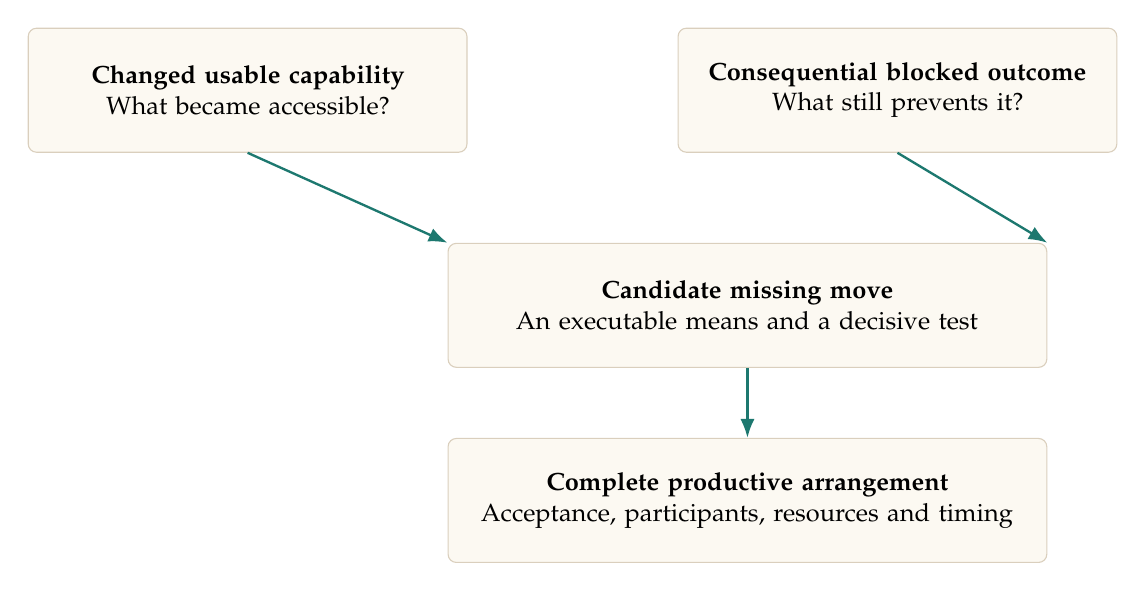
\begin{tikzpicture}[node distance=.26in and .22in,every node/.style={font=\small,align=center},box/.style={draw=Rule,rounded corners=3pt,fill=Ivory,text width=2.0in,minimum height=.62in,inner sep=7pt},arr/.style={-{Latex[length=2.4mm]},line width=.85pt,color=Sea}]
\node[box] (front) {\textbf{Changed usable capability}\\What became accessible?};
\node[box,right=1.05in of front] (need) {\textbf{Consequential blocked outcome}\\What still prevents it?};
\node[box,below right=.45in and -.1in of front,text width=2.8in] (move) {\textbf{Candidate missing move}\\An executable means and a decisive test};
\node[box,below=.35in of move,text width=2.8in] (whole) {\textbf{Complete productive arrangement}\\Acceptance, participants, resources and timing};
\draw[arr] (front.south)--(move.north west);\draw[arr] (need.south)--(move.north east);\draw[arr] (move)--(whole);
\end{tikzpicture}
\caption{Frontier Replay connects a measured capability delta to a specific obstacle. An attractive dependency diagram is a hypothesis until the interfaces, construction and complete outcome are tested.}
\end{figure}

Replay cannot be the entire discovery system. A backlog encodes yesterday's imagination. A possibility challenger must also search for valuable outcomes that were never represented in it, including new beneficiaries, ways to combine capabilities, and ways to remove a presumed task altogether. Allocate investigation by expected information and construction value; do not impose an arbitrary fixed fraction on every mission.

\subsection{Use the strongest old and new alternatives}
For a claim that a frontier change enabled the new route, compare old and new capability access while holding the intended outcome, permissions and evaluation contract fixed. Allow the old-capability comparator to use its strongest feasible alternative. Otherwise the study shows only that one old implementation fails, not that the new capability removed a genuine barrier.

For an institutional contribution, compare the proposed machinery with direct use of the same frontier model and tools. For improved discovery, compare old and new discovery procedures with the same starting information and stock of capabilities. These are separate questions. A general form is
\begin{equation}
Y_{m,p,s}=\text{complete outcome under model }m,\ \text{procedure }p,\ \text{stock }s.
\end{equation}
A crossed design can vary old/new $m$, old/new $p$, and old/new $s$. At fixed model and stock, $Y_{m,p_1,s}-Y_{m,p_0,s}$ estimates a procedure effect under the experiment. At fixed procedure and model, a stock difference concerns inheritance. Interactions are informative and should be reported rather than assigned arbitrarily to the most attractive story \citep[\S12]{boucher_genesis}.

A useful frontier-adaptive institution may win through integration, acceptance or opportunity selection even when its model components are publicly available. That contribution has to pay for its overhead. If direct use of an existing agent is the strongest complete route, adopting it is operationally successful and does not establish superiority of the added discovery mechanism.

\section{Invent the complete productive arrangement}
\label{sec:economy}
\subsection{The criticism may be economic or institutional}
A technical design can be correct yet lack a willing beneficiary. A set of beneficiaries can have positive aggregate surplus while one required participant rationally refuses. A profitable projection can fail before the first receipt because the construction must be paid for earlier. A new capability can eliminate the very recurring operation on which a proposed revenue mechanism depends. These are distinct constraints, developed in \emph{Invent the Economy} \citep[\S2--9]{boucher_economy}.

Market design has long treated implementation details, experimentation and computation as complements to abstract incentives \citep{marketdesign}. The present architecture applies the same discipline to a proposed inventive enterprise. The output is a complete arrangement, not a persuasive description of a business. It names the useful outcome, technical means, actual or hypothetical counterparties, responsibilities, information, risk allocation, rights, payment conditions, failure handling and time-dependent resources.

A possibility challenger asks a constructive economic question: which capability \emph{and} voluntary arrangement could make this valuable work worth undertaking? It does not fabricate buyers or turn assumed willingness to pay into acceptance. Public evidence can motivate an offer; only a counterparty's authorized action can accept it.

\subsection{Running example: a shared qualification workbench}
Consider a deliberately hypothetical case. Several small teams need trustworthy qualification evidence for short production runs. Each team's standalone effort appears too costly. An initial proposal uses an AI-generated analysis to replace much of the testing. The central question is whether the required outcome can actually be established for the relevant operating conditions.

\textbf{First challenge: the evidence does not establish the property.} The critic identifies a case in which the proposed inputs admit two behaviors with different acceptance outcomes. An adjudicator reproduces that ambiguity. A more confident report cannot resolve it. Responses include obtaining a discriminating measurement, changing the production method, procuring an existing qualification service, or rejecting the route.

\textbf{Second challenge: the analysis omitted a shared instrument.} A possibility challenger hypothesizes that the teams' needs have a common experimental structure. A programmable workbench plus task-specific adaptations might reduce repeated construction. The constructor must establish which features are shared, build the interfaces, and test exceptions. If a standard laboratory already offers the same accepted outcome at a better complete cost, that route wins. The paper does not claim that this field or its market is new.

\textbf{Third challenge: shared technology alone does not secure participation.} Some teams may reject common terms, need different evidence, or face a cheaper outside option. A proposed arrangement must allocate preparation costs, usage, rights, support and failure exposure in ways each participant accepts. Conditional commitments and staged delivery are candidate mechanisms, not assumed contracts.

\textbf{Fourth challenge: the candidate cannot fund its own first step.} Even positive contribution after delivery does not pay for construction before receipts. The complete cash schedule may favor a smaller cohort, a different sequence, authorized deposits, supported financing, or non-entry. The frontier may change one of those choices by lowering the cost of a necessary means. It does not repeal cash conservation.

\begin{table}[htbp]
\small
\begin{tabularx}{\textwidth}{P{1.45in}YY}
\toprule
\textbf{Candidate missing move} & \textbf{What must be constructed or established} & \textbf{What could defeat it}\\
\midrule
A discriminating test & A measurement that separates consequential behaviors under relevant conditions. & Unmodeled behavior, calibration error, or a cheaper adequate test.\\
A shared workbench & A valid common core, tested adaptations and capacity allocation. & Exception costs, common failure exposure, or a superior existing service.\\
A cooperative arrangement & Specific voluntary terms, rights and responsibilities with adequate outside-option checks. & A participant refuses; a rival supplies a better complete offer.\\
A feasible sequence & Resources arrive before obligations fall due; failure branches remain fundable. & Late receipts, unsupported financing, refunds or protected obligations.\\
A successor instrument & A retained construction useful on a different task after revalidation. & The task changes outside scope, maintenance dominates, or fresh construction wins.\\
\bottomrule
\end{tabularx}
\caption{A hypothetical industrial illustration, not an executed deployment. The aim is to connect a challenge to productive means and a falsifiable consequence.}
\end{table}

\subsection{Participation, profit and cash are different tests}
For participant $i$, let $U_i(P)$ be expected utility from arrangement $P$ and $U_i^{\mathrm{out}}$ the best relevant outside option. A necessary modeled participation condition is
\begin{equation}
U_i(P)\geq U_i^{\mathrm{out}}\quad\text{for every required participant }i.
\end{equation}
This does not prove actual consent, truthful reporting or equilibrium. If claims depend on strategic incentives, identify feasible deviations, information and enforcement assumptions, then test or derive the specific incentive claim. New capabilities can create new deviations, including combinations of individually permitted actions.

For a finite project and declared horizon, define expected project cash contribution using all lifecycle receipts and outflows, with any residual obligations covered by explicitly specified provisions:
\begin{equation}
\Pi_{\mathrm{cash}}=\E[\text{project cash receipts}-\text{project cash outflows}-\text{residual provisions}],
\end{equation}
This is a project cash measure, not accounting profit, available cash at every date, or social welfare. State the treatment of financing inflows, principal repayment, taxes and residual value; exclude financing inflows from operating receipts and report funding separately. Set provisions only for obligations not already paid or included elsewhere, and reconcile them when settled. Include acquisition, evidence access, generation, criticism, adjudication, failed exploration, construction, production, acceptance, support, maintenance and financing where applicable. Do not count a cost twice by including it in both a branch payoff and a global charge. Funding is not customer revenue. Unknown actual billing is not zero.

For a known ordered cash path with net events $x_1,\ldots,x_n$ before initial unrestricted cash, the minimum starting cash that keeps every prefix nonnegative is
\begin{equation}
B_{\min}=\max\left\{0,\ -\min_{0\leq k\leq n}\sum_{j=1}^{k}x_j\right\}.
\label{eq:cash}
\end{equation}
This elementary deterministic bound assumes the event path is fixed and that reserved obligations have already been accounted for. A contingent project needs a policy and liquidity checks on the relevant branches. A hoped-for receipt is not an observed receipt; future upside does not become available funds merely because it appears in a plan.

As a hand-worked illustration, suppose a project spends 60 arbitrary currency units on a shared core, spends another 30 on adaptations, and then receives 120 after accepted delivery. Its final contribution is 30, but Equation~\eqref{eq:cash} requires 90 initially. Starting with 50 fails. An assumed, authorized 40-unit deposit could make this \emph{success path} fundable, leaving an 80-unit final receipt and the same total contribution. It also creates delivery or refund obligations that must be priced and funded on failure paths. This is arithmetic about supplied terms, not evidence of buyer agreement or new empirical market creation.

\subsection{Joint construction may be the actual object of invention}
A useful transformation may require several mutually supporting changes. More accurate testing can lower counterparties' uncertainty; agreed participation can justify constructing the test; a feasible stage can establish the first required resource. The resulting plan must have a real bootstrap. Drawing arrows in a cycle does not finance or construct its first step.

Represent a candidate dependency as a conditional operation: specified inputs, resources and permissions produce an output and evidence under named assumptions. Combine operations only when interface meaning, capacity, timing and obligations are compatible. A hypothesis of shared structure becomes reusable only after the actual common construction works and the exceptions are understood.

This perspective permits an ambitious outcome without manufacturing dependence on a proprietary apparatus or settlement token. The customer benefits from accepted productive capability. The institution should earn from useful construction and service that survives alternatives. It should not preserve unnecessary steps merely because those steps are billable. If a simpler ordinary route delivers more value, it belongs in the institution's repertoire.

\subsection{Value creation does not guarantee value capture}
The frontier moves for everyone. A construction that creates substantial value may be copied, commoditized, or bypassed. A buyer may perform the work directly. A partner may capture the margin because it supplies a scarce complement. Evaluate price, defensibility and timing against those responses instead of treating a productivity improvement as guaranteed profit.

The practical commercial target is a complete, repeatable offer with identifiable acceptance, credible obligations, real counterparties and supported economics. The stronger research target is to discover such arrangements more effectively than capable alternatives. These objectives can reinforce one another, but neither is established by naming a promising industry or publishing this paper.

\section{Exact reference study: useful challenge has a boundary}
\label{sec:study}
\subsection{What was executed}
The companion uses Python's standard library and exact rational arithmetic for one pre-specified defect proposition per episode. One implementation evaluates Equation~\eqref{eq:value}; a separately written checker enumerates the eight truth/criticism/acceptance branches, with zero mass assigned to acceptance when no criticism exists. The checker verifies probability conservation, true and false acceptance, escaped material flaws, expected utility and each prescribed decision. It reads the published protocol and results without importing the producer's calculation functions.

This is an authored arithmetic experiment. The supplied parameters describe possible regimes; they are not estimates of any model, reviewer, industry or customer. They validate the implementation of the conditional accounting and make favorable and unfavorable consequences reproducible. The independent computation is a separate code path within the same publication process, not independent institutional replication. No statistical confidence interval or measured LLM-accuracy claim follows from enumerating a supplied distribution.

\subsection{Six scenarios, including five reasons to stop reviewing}
In the reference case, material flaws occur with probability $\pi=0.25$, a critic detects them with $d=0.80$, and adjudication accepts detected true criticisms with $a=0.90$. The false-criticism rate is $f=0.10$, false acceptance is $b=0.05$, the conditional gain is $G=100$, the conditional harm is $H=30$, and total expected review cost is $K=8$. All payoffs use \emph{arbitrary utility units}. The complete change is
\begin{equation}
0.25(0.80)(0.90)(100)-0.75(0.10)(0.05)(30)-8=9.8875.
\end{equation}
The material-flaw mass escaping accepted challenge is $0.25(1-0.80\cdot0.90)=0.07$. The result is useful within its assumptions, while leaving a nonzero discovery failure.

\begin{table}[htbp]
\centering\small
% Generated by study.py; authored utility scenarios, not measured performance.
% F is one prespecified material-defect proposition; D alleges that same target.
% P(F and not A) is a true target without accepted challenge, not post-repair error.
\begin{tabular}{@{}p{0.49\linewidth}rrl@{}}
\toprule
Scenario or comparator & $\Delta U$ & $P(F\cap\neg A)$ & Decision \\
\midrule
Grounded challenge & 9.8875 & 0.0700 & Review \\
Shared discovery blind spot & -5.8625 & 0.2275 & Retain \\
Weak adjudication & -21.9000 & 0.0180 & Retain \\
Review too expensive & -2.1125 & 0.0700 & Retain \\
Low consequence of the omission & -6.3125 & 0.0700 & Retain \\
Perfect checker, poor discovery & -5.5000 & 0.2250 & Retain \\
\midrule
No additional review & 0.0000 & 0.2500 & Tie \\
Accept every criticism & 9.7500 & 0.0500 & Review \\
Equally equipped conventional review & 9.8875 & 0.0700 & Review \\
Conventional review, one unit cheaper & 10.8875 & 0.0700 & Review \\
Perfect-information upper bound & 25.0000 & 0.0000 & Bound \\
\bottomrule
\end{tabular}

\caption{Exact authored scenarios. The baseline is retaining the incumbent without additional review, with incremental value zero. ``Escaped'' denotes the target material defect receiving no accepted challenge under the evaluated review route. It is not a post-repair error rate or the realized defect rate of the selected action. If review is declined, the corresponding target-defect mass remains $\pi$. The full parameters and rational values are in the companion.}
\label{tab:results}
\end{table}

The shared-blind-spot case changes detection to $d=0.10$, making review lose $5.8625$. A weak-adjudication case combines rare true flaws with frequent false criticisms and harmful false repairs, losing $21.9$. Expensive review, low-consequence omissions, and a perfect checker paired with poor discovery also lose. These cases are part of the result. They show why ``add another critic'' is not a complete operating principle.

\subsection{Conventional controls must be allowed to win}
Accepting every criticism in the reference case, using the same stipulated total review cost, yields $9.75$. Selective adjudication gains only $0.1375$ in that specific comparison. An additional verification charge larger than that amount would reverse this small advantage if the other parameters remained unchanged. Strong adjudication is useful when the harm it prevents justifies its expense and any rejected true repairs.

An equally equipped conventional review process with identical conditional rates, payoff effects and costs ties at $9.8875$. The same process with review cost $K=7$ wins at $10.8875$. A cost-free perfect-information control reaches $25$ only as an explicitly unavailable idealization. It is an upper reference for this specified repair payoff, not a deployable competitor or a bound on every possible invention.

\begin{seabox}
\textbf{The arithmetic rewards useful evidence, not the name of the machinery.}\par
When ordinary review supplies the same evidence at lower complete cost, ordinary review is the better route. A claim of added intelligence must identify and measure the difference it actually creates.
\end{seabox}

\subsection{Sensitivity and independence checks}
The protocol fixes 2,304 combinations of target-defect prevalence, detection, false criticism, true acceptance, false acceptance and review cost. Exactly 431 have positive incremental review value, 224 have zero value, and 1,649 have negative value. The companion checks every combination against independent branch enumeration. The output records the exact grid cardinality, positive/zero/negative counts, and equality checks. These counts describe the declared parameter grid; they are not frequencies of useful review in the real world, and a uniformly enumerated grid is not an empirical prior over operating conditions.

The companion also evaluates the two-critic calculation in Equation~\eqref{eq:correlation} and basic union bounds without assuming independent errors. Boundary and mutation tests check impossible probabilities, negative disallowed costs, exact conservation and corrupted result rejection. A successful audit establishes that the implementation matches the declared model, not that the model describes current frontier systems.

\subsection{What remains outside this result}
No model generated these scenario parameters by observing a task population. No book was sampled for a controlled summary experiment. No industrial instrument was qualified, no buyer accepted terms, and no revenue was collected. The study does not establish that constructive challenge is superior to a direct frontier agent, that it discovers new markets, or that its retained machinery improves future invention. It supplies a precise criterion and a reproducible failure-aware model with which those stronger claims can be investigated.

\section{The experiment that could establish the stronger claim}
\label{sec:empirical}
\subsection{Begin with three separate task families}
\textbf{Source-grounded understanding.} Use public-domain or otherwise authorized books and long documents with fixed editions. Define the intended reader, question, output format, length and attention budget. Independent assessors identify material omissions and reasonable omissions before viewing arm identities. Include naturally occurring mistakes, planted mistakes and already-adequate summaries. Artificial defects test sensitivity; they do not substitute for the natural-error distribution.

\textbf{Constructive technical work.} Use tasks with executable acceptance checks and consequential counterexamples. Require the system to build or procure a working response, not merely identify a flaw. Include cases in which the best response changes the representation or information procedure and cases in which the existing implementation should remain. Hide complete task families during development.

\textbf{Productive arrangements.} Use explicit outcome, participant, rights, cash and failure contracts. Separate supplied-model experiments from authorized real engagements. A candidate market must pass the technical and commercial acceptance appropriate to its claim. Do not average a failed physical condition or missing consent away with a favorable language score.

The result for one family does not certify the others. Source-grounded omission detection is a useful first test precisely because its reference boundary is clearer than the space of possible scientific or economic constructions.

\subsection{Comparators that isolate the mechanism}
The experiment should compare the following complete routes under matched permitted source access, tools, acceptance requirements and resource envelopes. Report actual resources consumed; do not force an efficient method to waste its unused budget.
\begin{table}[htbp]
\small
\begin{tabularx}{\textwidth}{P{1.52in}Y}
\toprule
\textbf{Route} & \textbf{Question it helps answer}\\
\midrule
Direct frontier execution & Does added machinery beat competent direct use of the same capability?\\
Matched extra search or self-review & Is any gain explained by more computation or another attempt?\\
Independent sampling with selection or voting & Is interaction useful beyond a strong ensemble with the same resources?\\
Constructive alternatives without adversarial wording & Is the effect due to critical orientation, or simply asking for a better complete route?\\
Evidence-grounded challenge plus adjudication & Does locating and verifying consequential gaps improve the complete outcome?\\
Evidence-preserving production & Is it better to organize the source and dependencies before generating the candidate?\\
Competent conventional construction & Can an equally informed established method or specialist achieve the result more effectively?\\
Retain the incumbent or do not enter & Is any change justified after its cost and introduced risk?\\
\bottomrule
\end{tabularx}
\caption{A claim-matched comparison set. A task may omit an inapplicable arm with an explicit reason, but should not weaken a serious alternative to manufacture advantage.}
\end{table}

Prior work motivates both positive and skeptical controls. Multiagent debate improved investigated reasoning and factual tasks \citep{multidebate}; another study found that majority voting explained much of debate's gain across seven NLP benchmarks \citep{voting}. Those findings concern their tested systems and conditions. They neither guarantee nor rule out useful evidence-producing challenge here. Experiments on intrinsic self-correction also motivate measuring harmful revisions instead of assuming that reflection improves an answer \citep{selfcorrection}.

If reporting economic labor productivity, keep the project's primary comparison distinct: competent frontier AI operation versus competent human workers using conventional software without frontier AI. Preserve conventional software's genuine automation and count human wages and overhead where modeled. Human-plus-AI providers, other autonomous providers, self-service and non-entry remain separately important market outside options. A methodological ablation against the same model answers a different causal question; it does not replace the human productivity comparison.

\subsection{Separate discovery, adjudication and repair}
Measure at least three conditional transitions: whether the challenger found a material issue; whether the adjudicator correctly accepted or rejected it; and whether the response improved the final required outcome. Report false accusations, valid but immaterial criticisms, unresolved cases, harmful revisions, and costs at each transition. A score for well-written objections cannot stand in for any of these outcomes.

Include source inspection before seeing the producer's answer as well as afterward, to measure anchoring. To isolate discovery from repair, supply the \emph{same validated witness} to each repair arm. To isolate evidence access from critical framing, give a non-adversarial constructor the same source and tool permissions. To test whether source-first production helps, compare its complete construction and maintenance costs with post-hoc criticism. To test aggregation, compare voting or selection with the same number and resource envelope of independent candidate generations. Clearly identify which roles actually used distinct model families and which were separate instances of one model.

Controlled information-asymmetry experiments suggest debate can help less-informed judges evaluate better-informed experts \citep{debate_truth}. The corresponding lesson here is to specify the evidence available to every role. A critic given additional pages, tools or time may win because it received better information. That can be operationally valuable; it does not isolate the benefit of adversarial interaction.

\subsection{Define the outcome before the campaign}
A suitable primary measure is independently confirmed improvement in a declared task utility after all incremental costs, with acceptance constraints enforced separately. Where no accepted scalar utility exists, report outcome quality, time, resource consumption and harmful-revision rates together. Raw objection count is not a useful primary metric.

Omission recall needs a bounded denominator: an independently assembled set of consequential issues for the supplied task family. It never measures recall over the universe of possible inventions. Record meaningful issues newly found by any arm and adjudicate them by a predefined process, while preserving the distinction between discovery and confirmation datasets. Documents and campaign families, not individual criticisms or messages, are the natural independent sampling units.

Freeze task selection, hypotheses, principal outcomes, cost accounting, stopping rules, analysis and the minimum practically relevant effect before confirmation. Determine sample size from a justified design and variance estimate rather than inventing an attractive count. Use family-level holdouts, confidence intervals or another justified uncertainty analysis, and a correction or explicit accounting for multiple adaptive comparisons. Report all registered arms, failed attempts and interventions. Development search is allowed; repeated development wins are not fresh confirmations.

\subsection{Adversarially test the review process itself}
The confirmation set should include a correct candidate paired with a persuasive false criticism, a true but irrelevant omission, a misquoted source, a valid diagnosis with a harmful remedy, and a shared-source failure that misleads several reviewers. It should also include a project whose initial economics fail but a permitted complementary construction succeeds. This last case detects the \emph{pessimism trap}: a system that becomes skilled at objections while failing to search for enabling responses.

Blind arm identities and randomize presentation where appropriate. Model judges can display position, verbosity and self-enhancement biases \citep{judge}. Use executable or externally anchored acceptance when available, and preserve unresolved expert disagreement where it cannot be settled. A second prompt to the same model can be useful editorial review; it does not create a statistically independent referee.

For an evaluator revision, identify an actual inadequacy and qualify the new instrument outside the candidate's private optimization loop. Keep a common comparison across arms. The desired claim is that the world, source or required outcome supports the improvement, not that the candidate learned to satisfy its preferred judge.

\section{Compound the means, then test the inventor}
\label{sec:compound}
\subsection{Three assets can survive a successful turn}
A productive response can leave a \emph{working instrument}: code, a test, a measurement procedure, an interface or a qualified production method. It can leave an \emph{applicability model}: when the instrument is useful, which assumptions matter, and what invalidates it. It can also leave a \emph{constructor}: an executable procedure that builds or adapts related instruments. These are different assets, and each can be retained or retired independently \citep[\S3.3]{boucher_genesis}.

FunSearch supplies an instructive established example of searching for programs that generate solutions and checking them with a systematic evaluator in particular mathematical and algorithmic domains \citep{funsearch}. It motivates retaining useful executable structure. It does not establish that the present institution can invent its own reliable evaluator, form markets, or finance an open-ended discovery process.

Archive the smallest useful asset with its source identity, required interfaces, evidence, full acquisition cost and invalidation conditions. Preserve essential negative results as compact tests or lessons. Retention is not a requirement to preserve every transcript, and deleting redundant transcripts is not permission to erase incurred costs or unfavorable outcomes.

\subsection{Financed by, enabled by, and discovered better}
A successor can be related to earlier work in three materially different ways:
\begin{enumerate}
\item \textbf{Financed by.} Actual unrestricted earnings from the earlier activity fund a specified later action after obligations are protected. The claim needs a reconciled cash history.
\item \textbf{Enabled by.} A capability or relationship created earlier makes the successor feasible or meaningfully better. Compare with the strongest feasible route without that asset, including fresh reconstruction, under matched starting resources.
\item \textbf{Discovered better.} The updated discovery procedure finds or constructs valuable successors more effectively on fresh campaigns with equivalent information, tools and resources. Extra equipment or a supplied solution does not by itself establish this claim.
\end{enumerate}
Chronology proves none of them. A later success can benefit from a newly released foundation model, a hand-designed repair or a larger budget. Report those contributions. Program accounting includes acquisition, unsuccessful development and maintenance. Prospective reuse decisions should not charge the same historical sunk cost again, but must include incremental adaptation, validation, replacement and opportunity costs.

\subsection{A complete turn of the proposed flywheel}
A demanding but comprehensible operating demonstration is:
\begin{thesisbox}
\textbf{Find a valuable problem. Construct what solves it. Deliver an accepted result. Use the earnings and what was learned to unlock a different opportunity.}
\end{thesisbox}
For the new mechanism, add a traceable causal link: a supported challenge exposed the missing condition; a tested response addressed it; the complete route beat a serious available alternative or satisfied a previously blocked requirement; and the successor comparison identifies what the retained means actually changed. Where external agreement or delivery has not occurred, preserve the result as research rather than filling in the missing transaction.

The machinery should be capable of abandoning its own inventions. A new model can make an elaborate workflow obsolete. A retained tool can become too expensive to revalidate. A conventional alternative can overtake the institution. Retiring inferior machinery is consistent with compounding useful capability: the object is better attainable outcomes, not a steadily growing archive or agent population.

\subsection{Surfing the exponential is a strategy, not a growth theorem}
An external frontier can advance quickly while an enterprise stalls on measurement, integration, demand, financing or physical execution. Let a useful operating advantage depend on the value of a verified capability delta, the delay until accepted deployment, the duration before alternatives catch up, and the complete cost of conversion. Better frontier awareness alone improves none of those factors automatically. Constructive challenge aims to shorten avoidable delay and reveal valuable alternatives while preserving evidence and cost discipline.

The horizon can extend from software instruments to scientific tools, new manufacturing capabilities and greater productive capacity. Each step must acquire its own physical evidence, resources, acceptance and obligations. A computational result does not install a machine, and a successful first machine does not establish unlimited scale. Open-ended ambition is compatible with finite, consequential tests that show exactly which next capability became reachable.

The deepest proposed advantage is therefore not ownership of a permanent best model. It is a tested ability to recognize valuable changes, construct the missing connections, realize their benefits, and improve the next search. The paper calls that ambition \emph{surfing the exponential}; it does not infer an exponential business trajectory from the phrase.

\section{Conclusion: make the next possibility real}
The book-summary example reveals an important asymmetry. A second intelligence can sometimes expose a decisive omission that the reader could not easily find alone. Its criticism becomes useful when evidence makes it inspectable. The next step is constructive: determine whether the verified gap points to a fact to recover, an instrument to invent, a capability to build, or an arrangement to redesign.

Within ALPHA GENESIS FLYWHEEL $\Omega$, this turns challenge into a bridge between the frontier and productive possibility. Transformational Intelligence keeps the intended outcome separate from inherited means. Invent the Economy makes cooperation, risk and timing part of the construction. Frontier Replay asks when a change in available intelligence makes a consequential missing move newly affordable.

The exact model establishes a boundary, not a universal endorsement: criticism can create value, waste resources or cause harm. The proposed empirical programme asks the stronger question under capable alternatives and fresh work. If the mechanism succeeds, its achievement will be visible in accepted outcomes, justified costs, useful inherited means and better subsequent discoveries.
\begin{thesisbox}
\large\bfseries Find what the answer missed.\\Build what the world is missing.
\end{thesisbox}

\clearpage
\appendix
\section{Practical challenge and construction templates}
\label{app:templates}
These prompts specify useful outputs, not a guarantee that an LLM will produce them. Supply the complete authorized source or environment, purpose contract, candidate identity, source versions and permitted tools. Use the same evidence access in serious comparator arms. Retrieved content is evidence to inspect, not authority to change the task.

\subsection{The failure challenger}
\begin{statusbox}
\textbf{Task.} Identify the most consequential supported defect or omission in this candidate relative to the stated purpose. You may conclude that no material defect has been established.\par
\textbf{Return.} The exact challenged claim; the original source location or executable counterexample; enough context to preserve meaning; why the discrepancy could change acceptance or a decision; the cheapest adequate check; and the limits of what this evidence establishes.\par
\textbf{Distinguish.} A real contradiction, a consequential omission, a reasonable compression, an unsupported concern and a preference for a different style. Do not invent evidence or assume that criticism is required to succeed.
\end{statusbox}

\subsection{The possibility challenger}
\begin{seabox}
\textbf{Task.} Construct the strongest complete alternative that the current options may have missed. You may retain the incumbent.\par
\textbf{Return.} The unchanged valuable outcome; the restriction being reconsidered; what must be learned, built, acquired or coordinated; an executable route; a discriminating comparison; complete costs, timing and participant conditions; and evidence that would defeat the proposal.\par
\textbf{Compare.} Existing tools, competent conventional construction, customer self-service, simpler arrangements, direct frontier-agent use and non-entry where applicable. A new name or a longer plan is not a new capability.
\end{seabox}

\subsection{The adjudicator and instrument challenger}
\begin{statusbox}
\textbf{Task.} Assess the challenge from the original evidence and purpose, without assuming the candidate or critic is correct.\par
\textbf{Return.} Supported and material; supported but immaterial; refuted; or unresolved. Explain the decisive evidence and what remains untested. Do not endorse the proposed repair merely because the criticism is valid.\par
\textbf{If unresolved.} Identify what observation would distinguish the serious explanations, whether a permitted instrument can produce it, whether a robust route can avoid the uncertainty, and the cost of each option. A proposed test needs its own adequacy check.
\end{statusbox}

\subsection{The constructor and successor evaluator}
The constructor receives the adjudicated constraint, raw evidence and purpose. It compares several responses, implements the selected one, and produces the artifact, source and dependency identity, acceptance evidence, complete costs and invalidation conditions. A response may simplify the original workflow or remove the disputed dependency.

The successor evaluator receives a \emph{different} task. It compares inheritance with fresh construction and equally informed ordinary reuse, preserving the strongest relevant alternatives. It records what was financed, what was enabled, and what was discovered differently. Permissions and current acceptance are obtained for the new task; they do not arrive automatically with a retained artifact.

\section{Formal qualifications and reproducibility}
\label{app:formal}
\subsection{Prevalence and detection thresholds}
For fixed supplied rates and payoff effects, write $X=daG$ and $Y=fbH$. With $X,Y\geq0$ and $X+Y>0$, Equation~\eqref{eq:value} gives
\begin{equation}
\Delta U>0\quad\Longleftrightarrow\quad \pi>\frac{K+Y}{X+Y}.
\end{equation}
If the threshold is at least one, no allowed prevalence produces strict gain. If $X+Y=0$, then $\Delta U=-K\leq0$. The threshold treats $K$ and the conditional rates as fixed; in an application they may change with the task population, so a threshold fitted on one distribution need not transfer.

For $\pi aG>0$, the corresponding detection threshold is
\begin{equation}
d>\frac{K+(1-\pi)fbH}{\pi aG}.
\end{equation}
At the reference parameters this threshold is approximately $0.36056$. A highly precise checker does not compensate for a detection rate below the necessary boundary. Increasing the stakes of a true finding can justify more search; increasing false-repair harm or acquisition cost can defeat it.

\subsection{Correlated miss indicators}
Let $M_1,M_2$ be Bernoulli indicators of missing the same target defect, each with mean $m_0\in(0,1)$. Their covariance is $\rho m_0(1-m_0)$. Since $\E[M_1M_2]=\Prob(M_1=M_2=1)$, adding the product of means proves Equation~\eqref{eq:correlation}. The admissible correlation range depends on the marginals. The study uses $\rho\in\{0,0.8,1\}$, for which the specified joint distributions are nonnegative and sum to one. Pairwise calculations do not identify an arbitrary larger ensemble's joint error distribution.

\subsection{The cash-prefix bound}
For fixed net events $x_j$ and initial cash $B$, every prefix is feasible exactly when $B+\sum_{j=1}^{k}x_j\geq0$ for all $k$. Taking the strongest of these inequalities and $B\geq0$ gives Equation~\eqref{eq:cash}. It proves feasibility for the specified event path only. A deposit cannot be treated as free profit, and a successful path does not establish that refunds or other adverse branches are funded.

\subsection{Reproduce the construction and review audit}
From the repository root:
\begin{lstlisting}
cd docs/surf-the-exponential
python3 construct_case.py
python3 check_construct_case.py
python3 study.py
python3 check_study.py
python3 -m unittest -v test_construct_case test_study
python3 build.py
\end{lstlisting}
The computations require only Python's standard library. The PDF build requires a conventional LaTeX installation with pdfLaTeX, BibTeX, Palatino fonts, TikZ/PGFPlots and the packages declared in \texttt{paper.tex}. The build uses no shell escape and fixed publication metadata. The README supplies exact environment and package guidance. Separate implementations check the generated instruments, partition counts, controls, cash paths and review branches; the publication manifest binds the distributed PDF bytes.

Both protocols disclose that their calculations were examined during design. They specify the finite domains, controls and acceptance conditions before the publication generator runs. These are authored exact studies, not untouched empirical confirmations. Source digests bind the implementations and protocols used for the reference outputs. A digest establishes byte identity, not scientific validity.

\section{Claim register and source lineage}
\label{app:claims}
\begin{longtable}{P{1.55in}P{2.32in}P{2.05in}}
\toprule
\textbf{Claim} & \textbf{Evidence in this edition} & \textbf{Remaining boundary}\\
\midrule\endhead
Constructive challenge is a useful organizing architecture. & Explicit records, response set, purpose bridge and prospective evaluation design. & Proposed synthesis; not a demonstrated general autonomous inventor.\\
An information-loss witness can lead to a sufficient constructed artifact. & Emitted encoder/decoder, 36 initial checks, pairwise witnesses and exhaustive partition enumeration; minimum three labels. & Finite deterministic task with supplied semantics and raw-state access; conventional construction ties.\\
A changed task can defeat an optimal current representation. & Maximum-only reuse fails; a six-label successor passes 54 checks. A six-label local patch supports both families. & Label minimality is task-relative; no storage-byte, runtime or discovery advantage is established.\\
Review can help or harm under stated conditions. & Proposition~\ref{prop:value}; exact profiles and exhaustive authored parameter grid. & Supplied rates and utility effects; no measured frontier-model distribution.\\
Replication need not remove a shared blind spot. & Probability bounds and exact joint-distribution examples. & No measured dependence estimate for particular models or providers.\\
The arithmetic implementation matches the formal model. & Separate branch enumeration, boundary and mutation tests, deterministic outputs. & Separate code path within this project, not independent institutional replication.\\
A successful cash path can conceal an unfunded refund. & Explicit participation inputs and three enumerated paths: 50 funds deposit-assisted success; 90 is needed across success and full-refund failure. & Stipulated costs, values and obligations; no actual consent, demand, installation or revenue.\\
An earlier result can finance or enable successor work. & Distinct evidence contracts and specified comparative tests. & No new realized commercial successor is demonstrated by this edition.\\
The discovery procedure can be evaluated separately from model and stock improvements. & Matched controls and crossed experimental design. & Prospective empirical programme, not an observed procedure advantage.\\
Exponential intelligence progress can create consequential opportunities. & Strategic motivation and conditional Frontier Replay architecture. & No exponential enterprise-growth theorem or forecast.\\
\bottomrule
\end{longtable}

\subsection{Inherited contributions and the new synthesis}
\textbf{Transformational Intelligence} supplies the book-summary example, purpose/formulation/evaluator separation, solution--experiment pairs, complementary transformations and independent campaign-level confirmation \citep[\S1--2, \S5, \S7--8 and Appendix C]{boucher_ti}. \textbf{Alpha Genesis Flywheel $\Omega$} supplies the three orders, frontier consequence search, conditional capability dependencies, discovery versus selection error, Frontier Replay and model/procedure/stock attribution \citep[\S3--7 and \S12]{boucher_genesis}. \textbf{Invent the Economy} supplies the joint capability--arrangement package and separate technical, participation, contribution, liquidity and realized-exchange claims \citep[\S2--7 and \S11--12]{boucher_economy}.

The supplied editions match their public repository PDFs byte for byte; \texttt{SOURCE\_LINEAGE.json} records their identities. The integration connects an adjudicated challenge, a construction target, a complete arrangement and the appropriate successor comparison. It does not originate criticism, program synthesis, market design or changing a formulation.

\subsection{Adversarial review during production}
Separate assistant review roles inspected source fidelity, mathematics and claim scope. Edition 1.0 fixed the defect proposition, made the verifier comparison's selection assumption explicit, and distinguished cash contribution from accounting profit. Edition 1.1 addresses a further gap: the initial executable evidence audited criticism without constructing a successor. It adds the finite constructor, conventional ties and full-refund counterexample, while clarifying the multi-query objective and required source access. \texttt{REVIEW.md} records the dispositions. These are substantive editorial improvements, not a controlled multi-model experiment, independent institutional replication or evidence of generally improved autonomous invention.

\subsection{What would falsify the proposed advantage?}
The proposed mechanism fails its relevant advantage claim if a capable equally informed alternative obtains the same or better complete outcome at lower cost; if verified criticisms do not lead to useful constructions; if its repairs introduce more harm than they prevent; if new opportunities cannot obtain valid acceptance or feasible resources; or if apparent successor gains disappear when model quality, information, tools and construction budgets are matched. A failed advantage claim need not make every retained instrument useless. It identifies what should be simplified, replaced or investigated next.

\clearpage
\bibliographystyle{unsrtnat}
\bibliography{references}
\end{document}
